% ═══════════════════════════════════════════════════════════════════════════════
% MARCO TEÓRICO - INSTITUTO ATENEO DE COLIMA
% Estudio Documental: Corrupción en México (2006-2012)
% ═══════════════════════════════════════════════════════════════════════════════

\nota{
  Este capítulo desarrolla el marco teórico-conceptual articulando doctrina 
  internacional (Nye, Rose-Ackerman, Klitgaard) con tradición académica mexicana 
  (Casar y Cejudo, Merino, Sandoval Ballesteros). La base conceptual sustenta el 
  análisis documental de los tres casos principales.
}

\section{Fundamentación teórica (autores y contribuciones)}

En las ciencias sociales y jurídicas no existe una definición única de corrupción, pero sí un consenso operativo que la conceptualiza como la desviación de deberes públicos o fiduciarios orientada a obtener beneficios indebidos en perjuicio del interés general \citep{inegi2016}. Con el propósito de sustentar rigurosamente el análisis de los casos seleccionados y elevar la densidad de la literatura científica arbitrada, la fundamentación teórica se articuló en seis ejes que vinculan teoría internacional con el pensamiento académico mexicano:

\begin{enumerate}
  \item \textbf{Fundamentos político-institucionales, económicos y tipificación internacional:} Desde la ciencia política, Joseph S. Nye (1967) define la corrupción como la conducta que se aparta de los deberes formales de un cargo público por consideraciones pecuniarias o de estatus privado ---personal, familiar o grupal---, o que infringe normas contra formas indebidas de influencia privada. En el plano económico-relacional, Susan Rose-Ackerman (1999, 2004) plantea el mal uso del poder público para beneficio privado o político como un fenómeno bilateral que germina en la interfaz entre el Estado (regulador o contratante) y el sector privado, actuando como un impuesto regresivo que encarece servicios, distorsiona licitaciones y frena la inversión productiva. A nivel normativo internacional, Transparencia Internacional adopta la noción ampliada de abuso de poder encomendado para beneficio propio, mientras que la Convención de las Naciones Unidas contra la Corrupción (CNUCC) tipifica el soborno (arts. 15, 16 y 21), el peculado (arts. 17 y 22), el tráfico de influencias (art. 18) y el abuso de funciones (art. 19) \citep{unodc2003}.

  \item \textbf{Corrupción sistémica, Estado capturado y rendición de cuentas en México:} La Oficina de las Naciones Unidas contra la Droga y el Delito (UNODC, s. f.) y María Amparo Casar y Guillermo M. Cejudo (2024) distinguen entre corrupción incidental ---actos aislados controlables por el sistema--- y corrupción sistémica, en la cual las transgresiones se normalizan y prevalece la impunidad. En la doctrina política mexicana, Mauricio Merino (2024) profundiza este diagnóstico bajo la categoría de Estado capturado, sosteniendo que la corrupción permeó el aparato público al punto de operar como regla que captura cargos, presupuestos y decisiones administrativas. Previamente, Sergio López Ayllón y Mauricio Merino (2009) demostraron que la rendición de cuentas no constituye un simple trámite contable, sino un sistema integral que requiere contrapesos horizontales entre poderes, vigilancia vertical ciudadana y capacidad efectiva de sanción. En consonancia, Jacqueline Peschard (2017) advierte que el acceso a la información y la transparencia resultan condiciones necesarias pero insuficientes para contener la corrupción cuando carecen de fiscalización autónoma y consecuencias jurídicas vinculantes.

  \item \textbf{Raíces organizacionales, históricas y concentración del poder:} Para explicar por qué la corrupción persiste pese a reformas legales sucesivas, la literatura mexicana aporta explicaciones organizacionales, históricas y culturales. Desde la teoría de las organizaciones, David Arellano Gault (2012, 2020) concibe la corrupción como una relación social densa ---expresada en redes informales de favores y lealtades--- incrustada en rutinas burocráticas, por lo cual las respuestas meramente punitivas o voluntaristas fracasan si no rediseñan incentivos y procesos administrativos. Desde la antropología histórica, Claudio Lomnitz (2000) muestra cómo en México se configuró una frontera porosa entre lo público y lo privado en la que lealtades familiares y clientelares compiten con la legalidad formal, sustentando las categorías de nepotismo y conflicto de interés. A su vez, Gabriel Zaid (2019) identifica la raíz del problema en la concentración discrecional del poder y en lo que denomina «la propiedad privada de las funciones públicas», insistiendo en cuantificar sus efectos con datos verificables.

  \item \textbf{Corrupción estructural, megainfraestructura, desigualdad y subrogación:} En la vertiente de economía política y contratación estatal, Irma Eréndira Sandoval Ballesteros (2009, 2024) formula la teoría de la corrupción estructural y el doble fraude, argumentando que los procesos de privatización, concesión y contratación pública sin controles efectivos permiten que élites políticas y económicas capturen las reglas institucionales con daños patrimoniales sistémicos. Complementariamente, Viridiana Ríos (2021) demuestra mediante evidencia cuantitativa que las reglas capturadas y la opacidad institucional amplifican la desigualdad económica al castigar desproporcionadamente a los hogares de menores ingresos. En materia de grandes obras, Cancino y el Banco Interamericano de Desarrollo (BID, 2020) ---retomando a Bent Flyvbjerg--- documentan patrones de fracaso en megainfraestructura asociados a decisiones políticas prematuras, subestimación de costos y opacidad en preinversión, mientras que Dávid-Barrett y Fazekas (2020) evidencian cómo la discrecionalidad contractual y la falta de candados transexenales exponen los proyectos estratégicos al favoritismo partidista. En el ámbito de servicios delegados, Bruno Rezzoagli et al. (2021) y el jurista mexicano José María Serna de la Garza (2010) acreditan que la subrogación y privatización sin capacidad regulatoria independiente diluyen la responsabilidad administrativa del Estado y multiplican el conflicto de interés.

  \item \textbf{Macrocriminalidad, seguridad pública y captura institucional en 2006--2012:} El análisis del aparato de seguridad durante 2006--2012 encuentra sustento directo en la teoría de la captura del Estado y la macrocriminalidad. Luis Daniel Vázquez Valencia (2019) explica cómo estructuras ilícitas coactúan con gobiernos formalmente constitucionales para vaciar instituciones democráticas y vulnerar derechos humanos, mientras que Luis Jorge Garay Salamanca y Eduardo Salcedo-Albarán (2012) diferencian entre Captura del Estado (CAE) y Reconfiguración Cooptada del Estado (RCDE). En la sociología política mexicana, Luis Astorga (2007, 2015) analiza la relación histórica entre poder político, cuerpos de seguridad y narcotráfico, dedicando un examen específico a las fallas institucionales y la concentración de mando durante la presidencia de Felipe Calderón. Asimismo, Carlos Antonio Flores Pérez (2009) demuestra cómo la alternancia política sin una reforma policial integral ni controles efectivos posibilitó la penetración del crimen organizado en estructuras gubernamentales. Como respaldo documental de caso, la investigación periodística en formato libro de Diego Enrique Osorno (2010) complementa los expedientes jurídicos sobre las redes políticas y omisiones de supervisión en la tragedia de la Guardería ABC.

  \item \textbf{Derechos humanos, medición empírica, legitimidad y encuadre mediático:} Finalmente, la Comisión Interamericana de Derechos Humanos (CIDH, 2019), la CNDH (2019) y Anne Peters (en IIJ-UNAM, 2018) establecen que la corrupción vulnera derechos fundamentales y debe evaluarse por la magnitud del daño infligido a las víctimas. En México, Federico Reyes Heroles (2003) marcó el tránsito analítico de concebir la corrupción como un asunto moral («de los ángeles») a medirla objetivamente mediante indicadores y costos verificables («a los índices»). En la misma línea, Alejandro Monsiváis-Carrillo (2020) demuestra que la impunidad sostenida erosiona la legitimidad democrática, y Sola-Morales y Zurbano-Berenguer (2019) explican cómo el encuadre mediático (framing) y la espectacularización política distorsionan la jerarquía de los problemas públicos. En cuanto al horizonte preventivo, autores como Klitgaard (1988), Mungiu-Pippidi (2015) y la OCDE (2017) coinciden en que contener la corrupción exige reducir monopolios discrecionales, fortalecer contrapesos y consolidar sistemas de integridad pública.
\end{enumerate}

\section{Marco contextual: definiciones operativas y diagnóstico empírico}

\subsection{Definición de palabras clave}

Con el propósito de preservar rigor terminológico y distinguir entre delitos acreditados, faltas administrativas graves e ineficiencia gubernamental, en el reporte se emplearon las siguientes definiciones operativas:

\begin{table}[H]
\centering
\caption{Definición operativa de palabras clave de la investigación}
\label{tab:definiciones}
\small
\begin{tabular}{@{}p{3.5cm}p{10cm}@{}}
\toprule
\textbf{Concepto clave} & \textbf{Definición operativa} \\
\midrule
Corrupción & Abuso de un poder o cargo encomendado ---público o privado--- para obtener un beneficio indebido en perjuicio del interés general y las normas establecidas; articula abuso de poder, beneficio indebido y quiebre de la integridad \citep{transparencia2026,inegi2016}. \\
\addlinespace
Soborno o cohecho & Ofrecer, dar, solicitar o aceptar dinero, bienes o favores para que una autoridad ejecute u omita actos propios de sus funciones \citep{unodc2003}. \\
\addlinespace
Peculado o desvío de recursos & Apropiación o uso de fondos, bienes o recursos públicos para fines privados o distintos a los autorizados presupuestalmente. \\
\addlinespace
Tráfico de influencias & Utilización del cargo público o de relaciones con otros servidores públicos para inclinar decisiones administrativas, contrataciones o resoluciones en favor de terceros. \\
\addlinespace
Conflicto de interés & Situación en la que el juicio o desempeño imparcial de un servidor público se ve comprometido por intereses personales, familiares o de negocios \citep{lomnitz2000}. \\
\addlinespace
Captura del Estado & Proceso mediante el cual redes lícitas o criminales infiltran, cooptan y subordinan instituciones estatales clave para operar bajo amparo institucional e impunidad \citep{merino2024,vazquezvalencia2019}. \\
\addlinespace
Subrogación de servicios públicos & Delegación de la prestación de un servicio público estatal (como las estancias infantiles del IMSS) a operadores privados mediante concesiones sujetas a regulación y vigilancia del Estado \citep{leal2010,sernadelagarza2010}. \\
\addlinespace
Encuadre mediático (framing) & Selección y énfasis de determinados atributos o símbolos de un hecho público en medios y redes sociales, capaz de moldear la percepción social de causalidad y urgencia \citep{solamorales2019}. \\
\bottomrule
\end{tabular}
\end{table}

\subsection{Antecedentes de la investigación: panorama empírico y arquitectura jurídica}

La medición contemporánea de la corrupción en México combina índices internacionales de percepción agregada con encuestas nacionales de experiencia directa en trámites públicos \citep{reyesheroles2003,zaid2019}. En la Tabla~\ref{tab:indicadores} se sintetizaron los indicadores secundarios oficiales más recientes y su contraste longitudinal con el cierre del sexenio 2006--2012:

\begin{table}[H]
\centering
\caption{Indicadores oficiales de percepción, prevalencia y costo de la corrupción en México (2012--2026)}
\label{tab:indicadores}
\small
\begin{tabular}{@{}p{2.8cm}p{2.5cm}p{3.5cm}p{4cm}@{}}
\toprule
\textbf{Indicador} & \textbf{Fuente / Edición} & \textbf{Resultado en México} & \textbf{Contexto y relación longitudinal (2012--2026)} \\
\midrule
Índice de Percepción de la Corrupción (IPC) & Transparencia Internacional (IPC 2025, publ. feb. 2026) & 27 / 100 puntos (Posición 141 de 182 países) & Descenso de siete puntos respecto a los 34 puntos del cierre de 2012; último lugar de la OCDE y por debajo del promedio de América (42 pts.). \\
\addlinespace
Percepción de frecuencia & INEGI --- ENCIG 2025 (publ. mayo 2026) & 84.1\,\% de la población adulta urbana & Percibió actos de corrupción gubernamental como frecuentes o muy frecuentes; brechas estatales de 89\,\% (Michoacán, BC, CDMX) a 67\,\% (Querétaro). \\
\addlinespace
Prevalencia en trámites y servicios & INEGI --- ENCIG 2025 & 15.6\,\% (15,642 actos por cada 100 mil hab.) & Proporción de usuarios que enfrentaron al menos un acto de corrupción al gestionar trámites; únicamente 21.7\,\% de las interacciones fueron digitales. \\
\addlinespace
Costo económico directo & INEGI --- ENCIG 2025 & \$17,707.4 millones de pesos anuales & Equivalente a \$3,865 pesos promedio por víctima; representó el costo real más elevado en la última década \citep{imco2026}. \\
\addlinespace
Satisfacción y confianza institucional & INEGI --- ENCIG 2025 & 47.2\,\% satisfacción en servicios; 23.9\,\% confianza en partidos & Disminución frente al 50.0\,\% de 2023; el transporte público (36.9\,\%) y el IMSS (43.3\,\%) obtuvieron las menores evaluaciones, frente a 75.9\,\% de confianza en universidades públicas. \\
\bottomrule
\end{tabular}
\end{table}

% FIGURA PENDIENTE
\begin{figure}[H]
\centering
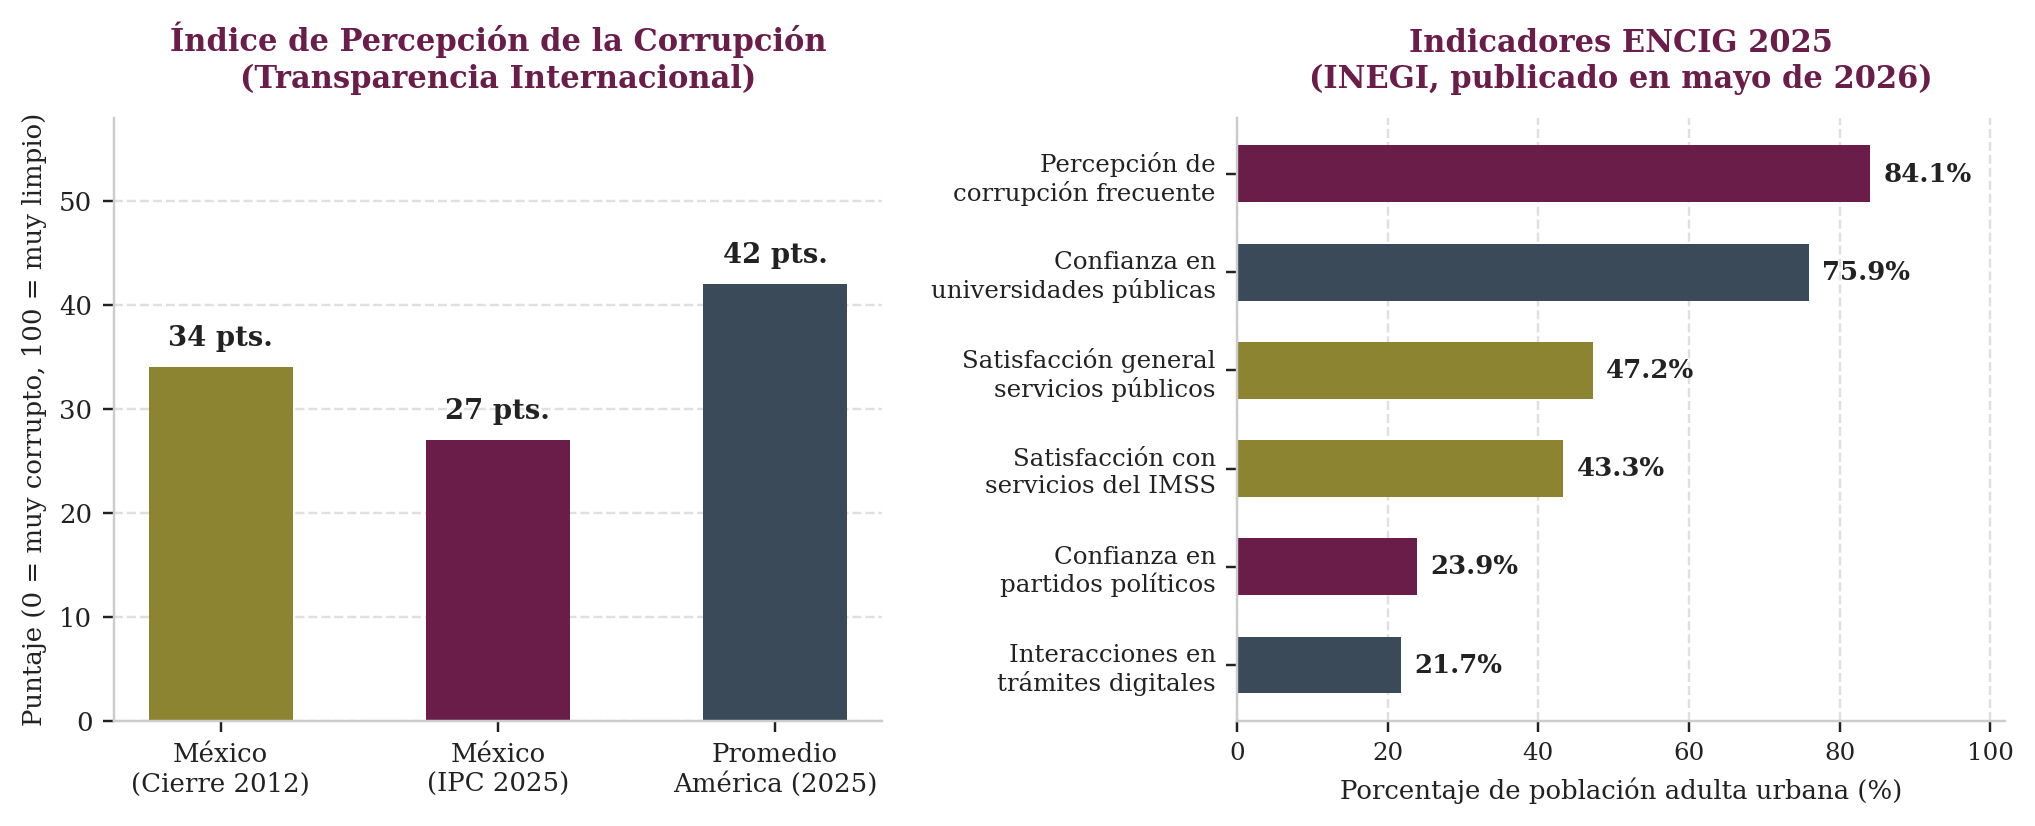
\includegraphics[width=0.9\textwidth]{img/image3.png} % Figura 1: Evolución IPC 2012 vs 2025 + ENCIG 2025
\caption{Evolución del Índice de Percepción de la Corrupción (2012 vs. 2025) e indicadores nacionales de la ENCIG 2025. Fuente: Elaboración propia con datos de Transparencia Internacional (2026) e INEGI (2026).}
\label{fig:ipc-encig}
\end{figure}